\documentclass{article}
\usepackage{amsfonts}
\usepackage{amsthm}
\usepackage{amssymb}
\usepackage{amsmath}
\usepackage{graphicx}
\usepackage{subcaption}

\newcommand{\new}[1]{
    \vspace{2mm}
    \noindent
    \textbf{
    \underline{#1}}
}

\def\calO{{\mathcal{O}}}
\def\th{{\theta}}
\def\_{{\hspace{1mm}}}
\def\<{{\langle}}
\def\>{{\rangle}}


\newcounter{problemcnt}
\setcounter{problemcnt}{0}

\newcommand{\Problem}{{
    \vspace{5mm}
    \stepcounter{problemcnt}
    \noindent
    \arabic{problemcnt}. 
}
}

\newcommand{\nProblem}[1]{
    \vspace{5mm}
    \noindent
    \setcounter{problemcnt}{#1}
    \arabic{problemcnt}. 
    \stepcounter{problemcnt}  
}


\newcommand{\Proof}{{
    \vspace{2mm}
    \noindent
    \textbf{
    \underline{Proof}}
}
}

\newcommand{\textOr}{
    {
        \hspace{5mm}
        \textrm{or}
        \hspace{5mm}
    }
}

\begin{document}
\begin{center}
\LARGE
PHYS 201 Problemset 9

\Large
Daniel Son
\end{center}

\normalsize

\nProblem{1}
Find the electromotive force induced 
on a square wire when the wire is passing 
through the center. 

\begin{center}
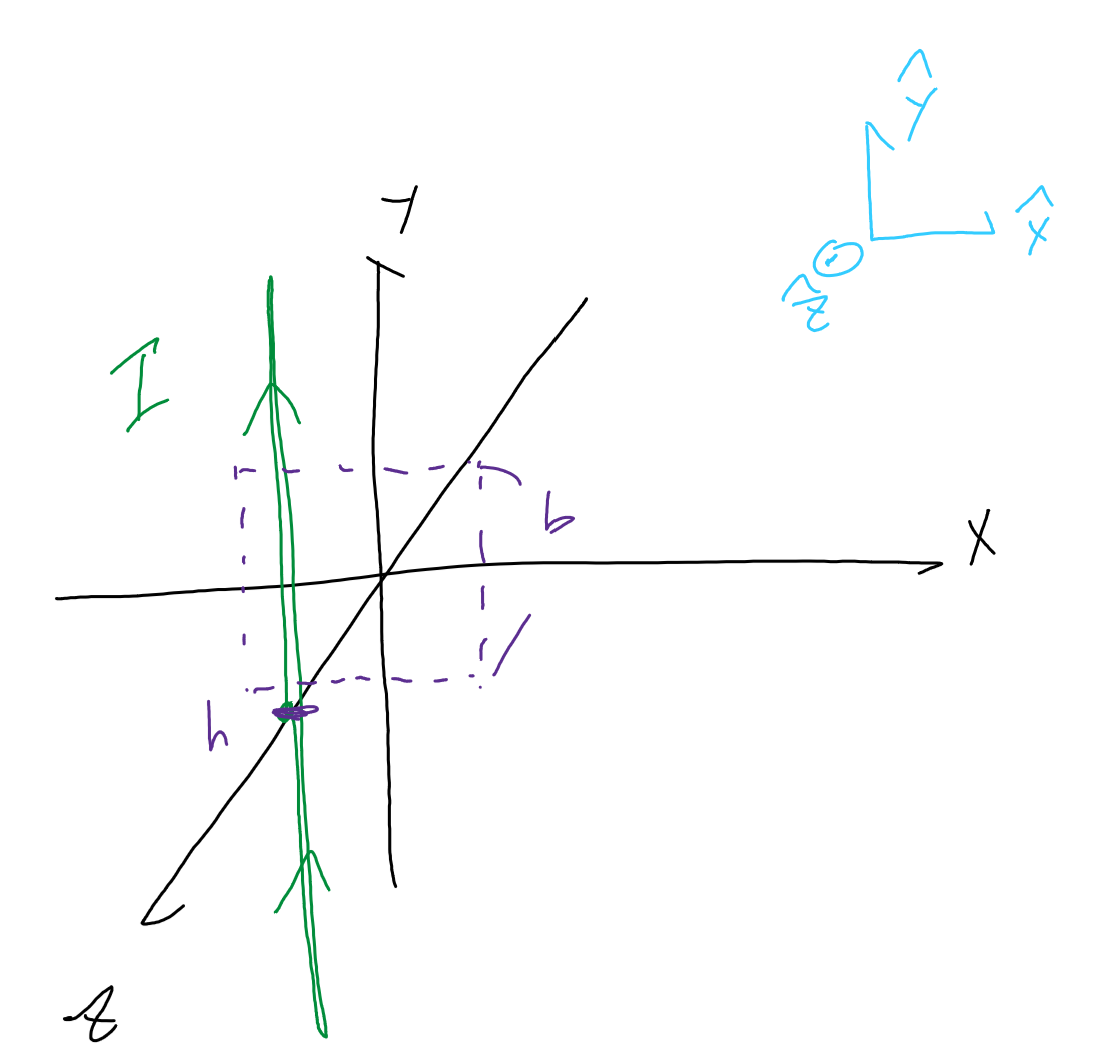
\includegraphics[width = .5\linewidth]{Q1_setup.png}

Figure 1: setup
\end{center}

To begin with, we determine the magnetic force 
along the xy-plane. Notice that by symmetry, 
the magnetic field is independent of the y 
axis. Thus, fix $y = z = 0$. We want to 
derive an equation for $\vec{B}(x)$. 

Recall:
\[
    B = 
    \frac{\mu_0I}
    {2\pi r}
\]
And that the direction of $B$ is determined 
by the right hand rule. We write:

\[
    \vec{B}(x) = 
    \frac{\mu_0 I}
    {2\pi \sqrt{x^2+h^2}}
    -\overline{{\<h, 0, x\>}}
\]

Where the bar denotes the unit vector. 
As to understand how the directional vetor is derived 
refer to the following figure:

\begin{center}
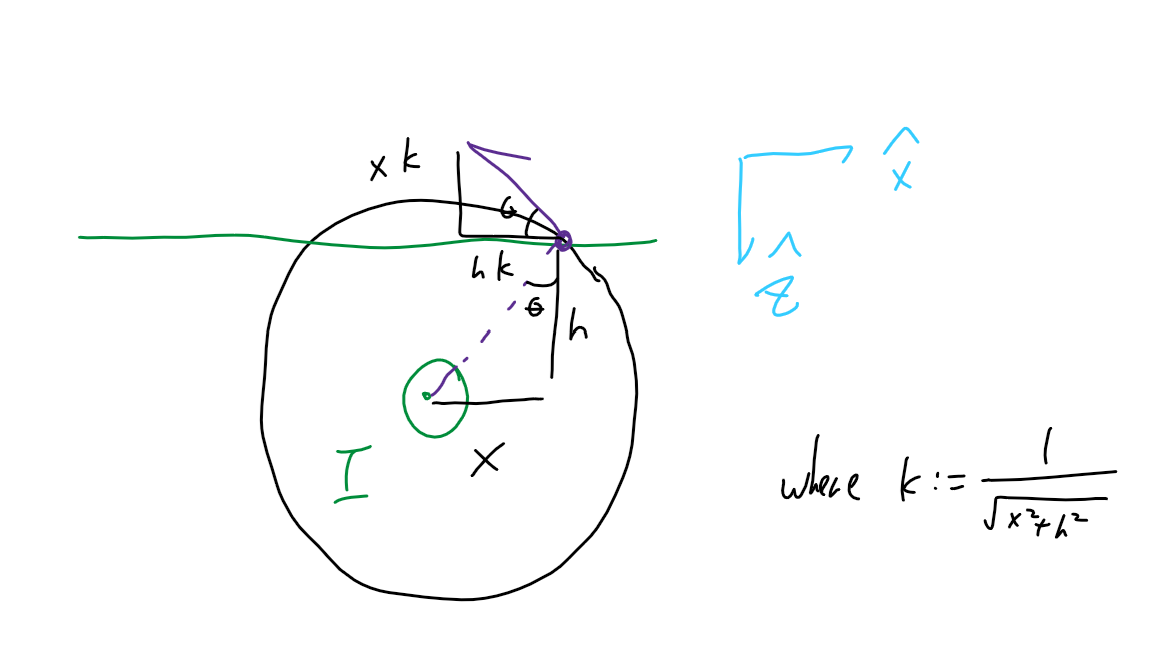
\includegraphics[width = .5\linewidth]{Q1_cut.png}

Figure 2: horizontal cut
\end{center}

Moreover, note that:

\[
    \vec{B}\cdot \vec{z} 
    = 
    \frac{\mu_0 I}
    {2\pi (x^2+h^2)}
    (-x)
\]

Now, compute the electromotive force 
by Faraday's Law. Write:

\def\EMF{{\mathcal{E}}}

\[
    \left.
    \EMF = 
    -
    \frac{d\Phi} {dt}
    \right|
    _{x = 0}    
\]

We can compute:
\[
    \left.
        \frac{d}{dx}
        \oint_{\gamma}
        \vec{B}d{\vec{a}}
    \right|_{x = 0}
    =
    b(\vec{B}\cdot\vec{z}
    \bigg|_{x = b/2}
    -\vec{B}\cdot\vec{z}
    \bigg|_{x = -b/2}
    )
\]

As we have established earlier, we write:
\[
    = b 
    \frac{\mu_0 I}
    {2 \pi (b^2/4+h^2)}
    \left[    
        -\frac{b}{2}
        -\frac{b}{2}
    \right]
    =
    -b^2
    \frac{\mu_0 I}
    {2 \pi (b^2/4+h^2)}
\]

By the chain rule:


\[
    \boxed{
    \left.
    \EMF = 
    -
    \frac{d\Phi} {dt}
    \right|
    _{x = 0}   
    =
    -
    \frac{dx}{dt}
    \left.
    \frac{d\Phi} {dx}
    \right|
    _{x = 0} 
    =
    \frac{2vb^2\mu_0I}{\pi(b^2+4h^2)}
    }
\]

\qed


\newpage

\nProblem{2}
A rod connected to a circuit 
is passing through a uniform magnetic 
field. Answer the following problems:
\begin{enumerate}
    \item When does the rod stop?
    \item How much has the rod traveled?
    \item What can be said about the energy of the system?
\end{enumerate}

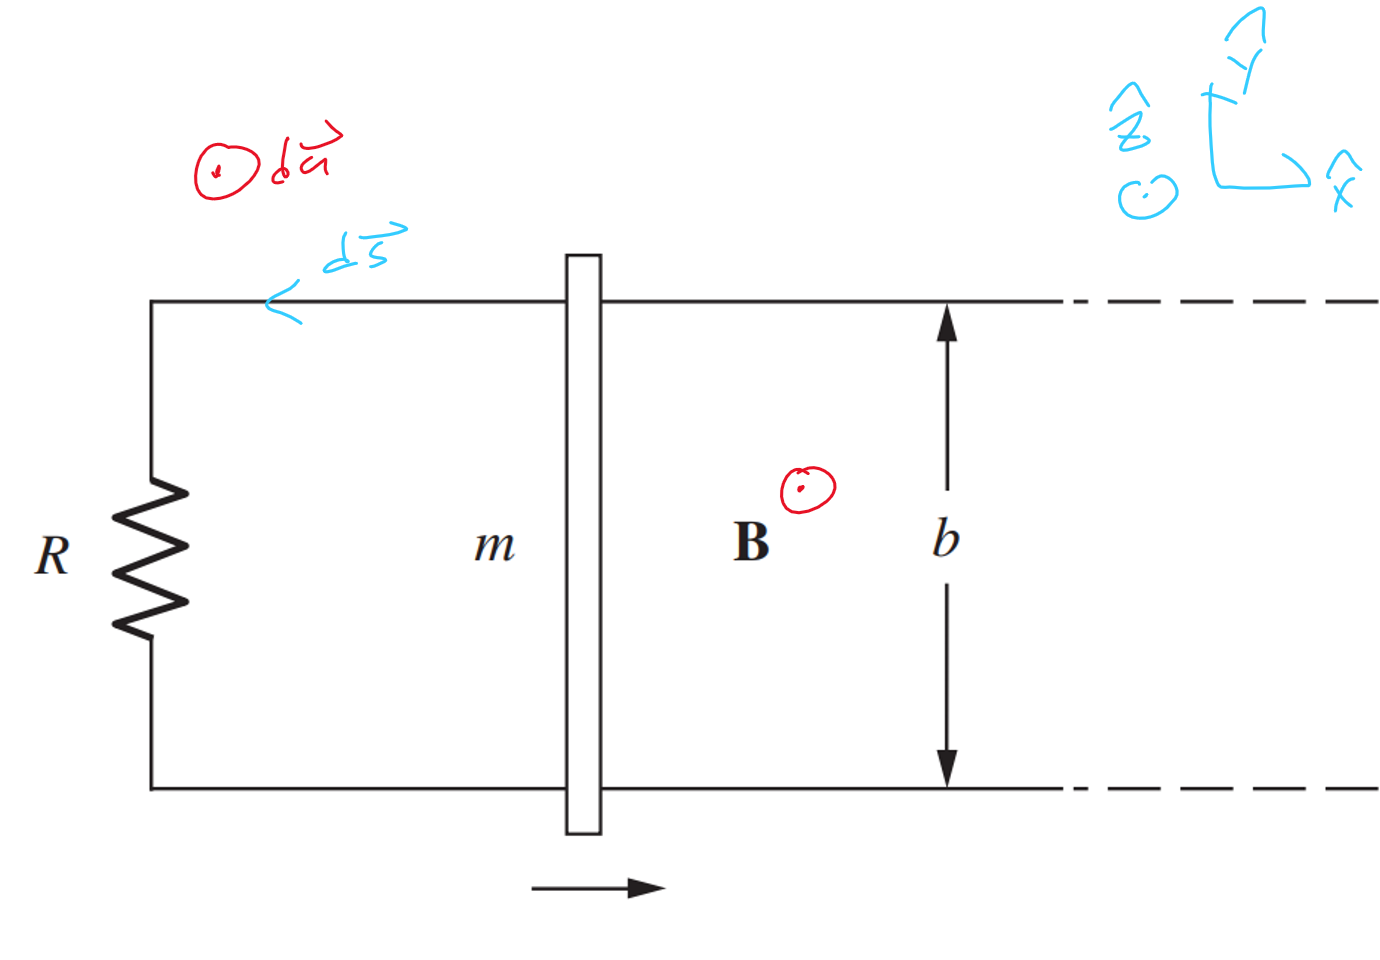
\includegraphics[width = .7\linewidth]{Q2_setup.png}

\new{Solution}
It seems reasonable to first come up 
with a time dependent equation of
the vertical velocity of the rod. Let 
$v(t)$ be a scalar function that describes 
the x direction velocity. Denote the initial 
velocity as $v_0$. 

We want to compute the current induced 
on the rod. The induced current 
will be perpendicular to the direction of 
the magnetic field. This in turn will 
create a Lorentz force that is opposite 
of the direction of movement. 

Define the direction of the surface vector 
$d\vec{a}$ to point out of the surface. 
Also, let $d\vec{s}$ to be counterclockwise. 

Now that all the directions are established 
move on to compute the integrals. To 
invoke Faraday's law, compute the magnetic 
flux. Write:

\[
    \Phi = \oint_{loop} \vec{B}d\vec{a}
     = lbB
\]

Where l denotes the horizontal distance 
from the resistor to the rod. 

By Faraday:

\[
    \EMF = 
    -\frac{d\Phi}{dt}
     = -vbB
\]
This derivative is justified by observing 
that the time derivative of $l$ is $v$. 

Apply Ohm's law to compute the current. 

\[
    \EMF = I R
\]
\[
    I = -\frac{vdB}{R}
\]

The current flows clockwise. 
Applying the right hand rule, 
we deduce that the magnetic field 
is towards the $-x$ direction. 

To compute the magnitude of the 
force exerted on the rod, consider
the following equation:

\[
    qv_{drift} = Ib
\]

where $q$ is the total moving charge 
inside the rod. 

Assuming that there is no electric field, 
we write:
\[
    F = qv_{drift}B
\]

We consider only the magnitudes, and 
$v_{drift}$, $B$ are perpendicular. Thus 
the equation is justified. Ignore self 
inductance. Also, $F = ma$. We write:

\[
    ma = IbB = \frac{vb^2B^2}{R}
\]
\[
    a = \frac{vb^2B^2}{mR}
\]
\[
    \frac{dv}{dt}
\]



\end{document}